
\documentclass[a4paper,12pt]{article}

%%% Работа с русским языком
\usepackage{cmap}					% поиск в PDF
\usepackage{mathtext} 				% русские буквы в формулах
\usepackage[T2A]{fontenc}			% кодировка
\usepackage[utf8]{inputenc}			% кодировка исходного текста
\usepackage[english, russian]{babel}	% локализация и переносы
\usepackage{indentfirst}
\frenchspacing
\usepackage{amsmath} 
\usepackage{amsfonts}
\usepackage{amssymb}

\newcommand{\bz}{\mathbf{z}}
\newcommand{\bx}{\mathbf{x}}
\newcommand{\by}{\mathbf{y}}
\newcommand{\bv}{\mathbf{v}}
\newcommand{\bw}{\mathbf{w}}
\newcommand{\ba}{\mathbf{a}}
\newcommand{\bb}{\mathbf{b}}
\newcommand{\bp}{\mathbf{p}}
\newcommand{\bq}{\mathbf{q}}
\newcommand{\bt}{\mathbf{t}}
\newcommand{\bu}{\mathbf{u}}
\newcommand{\bT}{\mathbf{T}}
\newcommand{\bX}{\mathbf{X}}
\newcommand{\bZ}{\mathbf{Z}}
\newcommand{\bS}{\mathbf{S}}
\newcommand{\bH}{\mathbf{H}}
\newcommand{\bW}{\mathbf{W}}
\newcommand{\bY}{\mathbf{Y}}
\newcommand{\bU}{\mathbf{U}}
\newcommand{\bQ}{\mathbf{Q}}
\newcommand{\bP}{\mathbf{P}}
\newcommand{\bA}{\mathbf{A}}
\newcommand{\bB}{\mathbf{B}}
\newcommand{\bC}{\mathbf{C}}
\newcommand{\bE}{\mathbf{E}}
\newcommand{\bF}{\mathbf{F}}
\newcommand{\bomega}{\boldsymbol{\omega}}
\newcommand{\btheta}{\boldsymbol{\theta}}
\newcommand{\bgamma}{\boldsymbol{\gamma}}
\newcommand{\bdelta}{\boldsymbol{\delta}}
%\newcommand{\bPsi}{\boldsymbol{\Psi}}
%\newcommand{\bpsi}{\boldsymbol{\psi}}
\newcommand{\bxi}{\boldsymbol{\xi}}
\newcommand{\bchi}{\boldsymbol{\chi}}
\newcommand{\bzeta}{\boldsymbol{\zeta}}
\newcommand{\blambda}{\boldsymbol{\lambda}}
\newcommand{\beps}{\boldsymbol{\varepsilon}}
\newcommand{\bZeta}{\boldsymbol{Z}}
% mathcal
\newcommand{\cX}{\mathcal{X}}
\newcommand{\cY}{\mathcal{Y}}
\newcommand{\cW}{\mathcal{W}}

\newcommand{\dH}{\mathbb{H}}
\newcommand{\dR}{\mathbb{R}}
% transpose
\newcommand{\T}{^{\mathsf{T}}}

\renewcommand{\epsilon}{\ensuremath{\varepsilon}}
%\renewcommand{\phi}{\ensuremath{\varphi}}
\renewcommand{\kappa}{\ensuremath{\varkappa}}
\renewcommand{\le}{\ensuremath{\leqslant}}
\renewcommand{\leq}{\ensuremath{\leqslant}}
\renewcommand{\ge}{\ensuremath{\geqslant}}
\renewcommand{\geq}{\ensuremath{\geqslant}}
\renewcommand{\emptyset}{\varnothing}

%%% Дополнительная работа с математикой
\usepackage{amsmath,amsfonts,amssymb,amsthm,mathtools} % AMS
\usepackage{icomma} % "Умная" запятая: $0,2$ --- число, $0, 2$ --- перечисление

%% Номера формул
%\mathtoolsset{showonlyrefs=true} % Показывать номера только у тех формул, на которые есть \eqref{} в тексте.
%\usepackage{leqno} % Нумереация формул слева

%% Свои команды
\DeclareMathOperator{\sgn}{\mathop{sgn}}

%% Перенос знаков в формулах (по Львовскому)
\newcommand*{\hm}[1]{#1\nobreak\discretionary{}
	{\hbox{$\mathsurround=0pt #1$}}{}}

%%% Работа с картинками
\usepackage{graphicx}  % Для вставки рисунков
\setlength\fboxsep{3pt} % Отступ рамки \fbox{} от рисунка
\setlength\fboxrule{1pt} % Толщина линий рамки \fbox{}
\usepackage{wrapfig} % Обтекание рисунков текстом

%%% Работа с таблицами
\usepackage{array,tabularx,tabulary,booktabs} % Дополнительная работа с таблицами
\usepackage{longtable}  % Длинные таблицы
\usepackage{multirow} % Слияние строк в таблице

%%% Теоремы
\theoremstyle{plain} % Это стиль по умолчанию, его можно не переопределять.
\newtheorem{theorem}{Теорема}[section]
\newtheorem{proposition}[theorem]{Утверждение}

\theoremstyle{definition} % "Определение"
\newtheorem{corollary}{Следствие}[theorem]
\newtheorem{problem}{Задача}[section]

\theoremstyle{remark} % "Примечание"
\newtheorem*{nonum}{Решение}

%%% Программирование
\usepackage{etoolbox} % логические операторы

%%% Страница
\usepackage{extsizes} % Возможность сделать 14-й шрифт
\usepackage{geometry} % Простой способ задавать поля
\geometry{top=25mm}
\geometry{bottom=35mm}
\geometry{left=35mm}
\geometry{right=20mm}
%
%\usepackage{fancyhdr} % Колонтитулы
% 	\pagestyle{fancy}
%\renewcommand{\headrulewidth}{0pt}  % Толщина линейки, отчеркивающей верхний колонтитул
% 	\lfoot{Нижний левый}
% 	\rfoot{Нижний правый}
% 	\rhead{Верхний правый}
% 	\chead{Верхний в центре}
% 	\lhead{Верхний левый}
%	\cfoot{Нижний в центре} % По умолчанию здесь номер страницы

\usepackage{setspace} % Интерлиньяж
%\onehalfspacing % Интерлиньяж 1.5
%\doublespacing % Интерлиньяж 2
%\singlespacing % Интерлиньяж 1

\usepackage{lastpage} % Узнать, сколько всего страниц в документе.

\usepackage{soul} % Модификаторы начертания

\usepackage{hyperref}
\usepackage[usenames,dvipsnames,svgnames,table,rgb]{xcolor}
\hypersetup{				% Гиперссылки
	unicode=true,           % русские буквы в раздела PDF
	pdftitle={Заголовок},   % Заголовок
	pdfauthor={Автор},      % Автор
	pdfsubject={Тема},      % Тема
	pdfcreator={Создатель}, % Создатель
	pdfproducer={Производитель}, % Производитель
	pdfkeywords={keyword1} {key2} {key3}, % Ключевые слова
	colorlinks=true,       	% false: ссылки в рамках; true: цветные ссылки
	linkcolor=red,          % внутренние ссылки
	citecolor=black,        % на библиографию
	filecolor=magenta,      % на файлы
	urlcolor=cyan           % на URL
}

\usepackage{csquotes} % Еще инструменты для ссылок

%\usepackage[style=authoryear,maxcitenames=2,backend=biber,sorting=nty]{biblatex}

\usepackage{multicol} % Несколько колонок

\usepackage{tikz} % Работа с графикой
\usepackage{pgfplots}
\usepackage{pgfplotstable}


\begin{document}

\title{Machine learning models for Navier-Stocks}
\author{Боева Галина, группа М05-304а}
\date{\today}

\maketitle
\section{Введение}
В этой статье мы заинтересованы в решении уравнений Навье-Стокса с использованием
метода машинного обучения, называемого нейронной сетью, основанной на физике (PINN). PINN включает физические
законы в архитектуру глубокого обучения, которая ограничивает возможные решения с помощью нейронной
сети. Использовании закрепленного за Навье-Стокса по-прежнему находится в зачаточном состоянии, и многие
вопросы для решения, например, наиболее подходящая форма физических законов. В данной статье исследуются
возможности PINN для решения уравнений Навье-Стокса в двух формулировках (скорость-давление
и тензор напряжений Коши) для решения трех контрольных задач, а именно: потока Пуазейля, потока
Куэтта и потока в полости, управляемой крышкой.

\section{Формулировки уравнений Навье-Стокса}

\cite{raissi2017physics} представили общую структуру PINN для моделирования сложных физических систем. Это исследование решило несколько случаев двумерного стационарного несжимаемого потока, включив уравнения Навье-Стокса в PINN. Естественный вопрос: какую формулировку уравнений Навье-Стокса следует использовать? Чтобы ответить на этот вопрос, мы сравнили производительность PINN с формами VP и ST уравнений Навье-Стокса.

\subsection{Форма скорость-давление (VP)}

Форма VP двумерных стационарных несжимаемых уравнений Навье-Стокса имеет вид:
\begin{equation}
\rho (u \cdot \nabla) u = -\nabla p + \mu \nabla^2 u \quad \text{в } \Omega
\end{equation}
\[
\nabla \cdot u = 0 \quad \text{в } \Omega
\]
\[
u = u_\Gamma \quad \text{на } \Gamma_D
\]
\[
\partial_n u = 0 \quad \text{на } \Gamma_N
\]
где $\nabla$ — оператор набла, $u = (u, v)$ — вектор скорости, $p$ — давление, $\mu$ — вязкость жидкости, $\rho$ — плотность жидкости. Граничные условия необходимы для решения уравнений, где $\Gamma_D$ и $\Gamma_N$ обозначают границы Дирихле и Неймана соответственно. В форме VP решения уравнений Навье-Стокса аппроксимируются глубокой нейронной сетью (DNN), которая принимает пространственные координаты в качестве входов для прогнозирования полей давления и скорости, т.е. $(x, y) \rightarrow (p, u, v)$.

\subsection{Форма тензора напряжений Коши (ST)}

Форма ST двумерных стационарных несжимаемых уравнений Навье-Стокса имеет вид:
\begin{equation}
\rho (u \cdot \nabla) u = -\nabla \cdot \sigma \quad \text{в } \Omega
\end{equation}
\[
\sigma = -pI + \mu (\nabla u + \nabla u^T) \quad \text{в } \Omega
\]
\[
\nabla \cdot u = 0 \quad \text{в } \Omega
\]
\[
u = u_\Gamma \quad \text{на } \Gamma_D
\]
\[
\partial_n u = 0 \quad \text{на } \Gamma_N
\]
где $\sigma$ — тензор напряжений Коши. Форма ST уменьшает порядок производных по сравнению с формой VP и увеличивает обучаемость DNN. Решения уравнений Навье-Стокса аппроксимируются DNN, которая принимает пространственные координаты в качестве входов и прогнозирует поля давления и тензор напряжений Коши, $(x, y) \rightarrow (p, \sigma)$, которые затем дифференцируются для получения скорости.

\section{Формулировки PINN}

По сути, PINN — это DNN с включенными в формулировку физическими законами. Первые слои в PINN — это стандартная прямая сеть, с входами и выходами, определяемыми пользователем в соответствии с управляющими уравнениями. Обратите внимание, что входы и выходы также зависят от формы управляющих уравнений. Физические законы, которые должны быть удовлетворены, входят в формулировку PINN на последнем слое. Веса PINN обучаются для минимизации функции потерь, которая включает потери данных, уравнений и граничных условий. В этой статье мы используем PINN для решения уравнений Навье-Стокса. Потери данных затем исключаются из уравнения, так как меченные данные недоступны. Наконец, потери уравнений и граничных условий объединяются в так называемые физические потери.

Функция физических потерь, $J_p$, для получения решений как для уравнения (1), так и для уравнения (2), определяется следующим образом:
\begin{equation}
J_p = J_g + \alpha J_{BC}
\end{equation}
\begin{equation}
J_g = \frac{1}{N_g} \sum_{i=1}^{N_g} r_g(x_i)^2
\end{equation}
\begin{equation}
J_{BC} = \frac{1}{N_{BC}} \sum_{i=1}^{N_{BC}} (u_i - u_i^{BC})^2
\end{equation}
где $J_g$ и $J_{BC}$ — потери управляющих уравнений и граничных условий соответственно. Мы оцениваем остатки управляющих уравнений на множестве точек, называемых точками коллимации. С другой стороны, потери граничных условий оцениваются на множестве граничных точек. Число точек коллимации и граничных точек обозначаются как $N_g$ и $N_{BC}$ соответственно. Затем $r$ — остаток предсказанного значения относительно управляющих уравнений. Наконец, $u$ и $u^{BC}$ — значения из DNN и заданных граничных условий в граничных точках соответственно. Кроме того, у нас также есть вес потерь, $\alpha > 0$, для контроля компромисса между $J_{BC}$ и $J_g$. 

\begin{figure*}
    \centering
    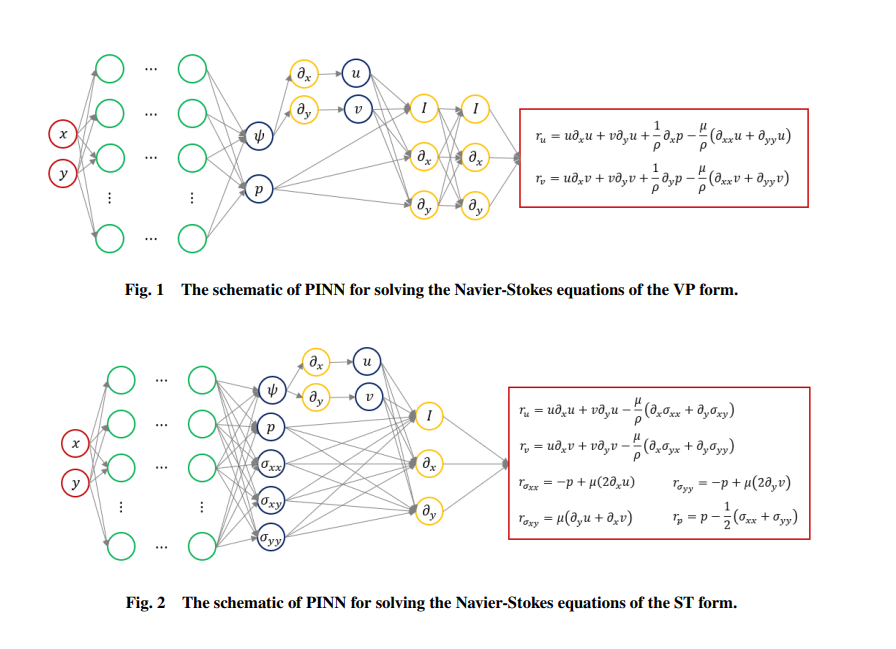
\includegraphics[width=0.85\linewidth]{image1.png}
    \caption{Caption}
    \label{fig:enter-label}
\end{figure*}
Схематическое изображение PINN для решения уравнений (1) и (2) показано на рисунках 1 и 2 соответственно. Решения уравнений Навье-Стокса определяются на основе рисунков 1 и 2 путем принятия пространственных координат в качестве входов и затем прогнозирования соответствующих полей скорости и давления, т.е. $(x, y) \rightarrow (u, v, p)$. Исходные выходы DNN — это $\psi$, $p$ или $\sigma$. Для решения управляющих уравнений мы выполняли автоматическое дифференцирование (AD), используя 'tf.gradients()' из TensorFlow, чтобы найти $u$, $v$ и другие производные термины.

Для обеих формулировок нелинейная функция активации — это гиперболический тангенс (tanh), который часто показывает лучшие результаты, чем логистическая сигмоида в многих приложениях~\cite{goodfellow2016deep}. Также хорошей практикой является использование инициализации весов Xavier Normal или Xavier Uniform и масштабирование входных данных до диапазона от -1 до 1 перед обучением~\cite{rodriguez2022choose}, когда используется функция активации tanh.

Производные соответствующих переменных в управляющих уравнениях вычисляются с использованием автоматического дифференцирования (AD)~\cite{baydin2018automatic}. Затем мы минимизировали функцию потерь, используя стохастический градиентный метод оптимизации ADAM~\cite{kingma2014adam} и метод оптимизации L-BFGS-B~\cite{byrd1995limited}. Основное преимущество использования ADAM — это адаптивная скорость обучения для ускорения сходимости~\cite{kingma2014adam} . Мы используем метод ADAM для получения лучшего набора весов нейронной сети для первых итераций, продолженный L-BFGS-B для получения более высокой точности~\cite{liu1989limited}.

Для автоматического контроля $\alpha$ в уравнении (3) мы также экспериментировали с динамической и адаптивной стратегией весов во время обучения сети, как предложил Wang и др. [12]. Формально, параметры нейронных сетей обучаются следующим образом:
\begin{equation}
\theta^{(k+1)} = \theta^{(k)} - \eta \nabla_\theta J_g - \alpha \nabla_\theta J_{BC},
\end{equation}
где $\theta$ представляет параметры PINN, а именно веса всех полносвязных слоев, $k$ обозначает шаг итерации, а $\eta$ — скорость обучения. Оценки $\alpha$ могут быть вычислены для каждого шага обучения, например, на $(k+1)$, следующим образом:
\begin{equation}
\hat{\alpha}^{(k+1)} = \frac{\max_\theta \{|\nabla_\theta J_g|\}}{|\nabla_\theta \alpha^{(k)} J_{BC}|},
\end{equation}
где $\max_\theta \{|\nabla_\theta J_g|\}$ — максимальное значение, вычисленное из $|\nabla_\theta J_g|$, а $|\nabla_\theta \alpha^{(k)} J_{BC}|$ обозначает средние значения $|\nabla_\theta \alpha^{(k)} J_{BC}|$.

Соответственно, коэффициенты взвешивания для следующей итерации обновляются с использованием формы скользящего среднего:
\begin{equation}
\alpha^{(k+1)} = (1 - \lambda) \alpha^{(k)} + \lambda \hat{\alpha}^{(k+1)}
\end{equation}
Коэффициент $\lambda$ в уравнении (8) — это гиперпараметр, определяющий, как быстро снижаются вклады предыдущих адаптивных весов. Меньшее значение $\lambda$ означает, что предыдущие значения вносят больший вклад в текущие динамические веса, что обеспечит стабильность регулировки во время обучения. В этой статье выбрано $\lambda = 0.1$.

\section{Математическая модель из статьи 2014 года}
В этой статье разработан новый метод, основанный на нейронной
сети, для получения решения уравнений
Навье–Стокса в форме аналитической функции.
Процедура решения основана на формировании пробного
решения, состоящего из двух частей. Первая часть непосредственно
удовлетворяет граничным условиям и, следовательно, не содержит
настраиваемых параметров. Вторая часть построена таким
образом, что основное уравнение выполняется внутри области решения
, в то время как граничные условия остаются неизменными.
Эта часть включает в себя нейронную сеть с прямой связью, содержащую настраиваемые параметры (веса), которые должны быть
определены таким образом, чтобы результирующая приблизительная
функция ошибки была сведена к минимуму. 
Двумерные уравнения Навье-Стокса, включая уравнения непрерывности и импульса, рассматриваются для несжимаемого ламинарного потока в безразмерной форме:
\[
\frac{1}{\text{Re}} \frac{\partial^2 u}{\partial x^2} = u \frac{\partial u}{\partial x} + v \frac{\partial u}{\partial y} + f_1 \quad \text{в } X
\]
\[
\frac{1}{\text{Re}} \frac{\partial^2 v}{\partial y^2} = u \frac{\partial v}{\partial x} + v \frac{\partial v}{\partial y} + f_2 \quad \text{в } X
\]
\[
\frac{\partial u}{\partial x} + \frac{\partial v}{\partial y} = 0 \quad \text{в } X
\]
где $X \subset \mathbb{R}^2$ — прямоугольная область, $u(x, y)$ и $v(x, y)$ — продольная и нормальная компоненты поля скорости соответственно, $f_1$ и $f_2$ — компоненты заданной внешней силы (например, гравитации).

Для двумерного потока можно ввести функцию потока $w(x, y)$:
\begin{equation}
u = \frac{\partial w(x, y)}{\partial y}, \quad v = -\frac{\partial w(x, y)}{\partial x}
\end{equation}
которая непосредственно удовлетворяет уравнению непрерывности. Исключение давления из уравнений импульса с использованием функции потока приводит к уравнению транспорта вихря:
\begin{equation}
\frac{1}{\text{Re}} \left( \frac{\partial^2 w}{\partial y^2} \frac{\partial w}{\partial x} - \frac{\partial^2 w}{\partial x^2} \frac{\partial w}{\partial y} \right) = \frac{\partial f_1}{\partial y} - \frac{\partial f_2}{\partial x}
\end{equation}
Уравнение (10) имеет единственное решение, если на $\partial X$ заданы два граничных условия.

Рассматриваются следующие два граничных условия на $\partial X$ для $w(x, y)$:
\begin{equation}
w(x, y) = g(x, y)
\end{equation}
\begin{equation}
\frac{\partial w(x, y)}{\partial n} = h(x, y)
\end{equation}
где $n$ — единичный вектор, нормальный к $\partial X$, $g(x, y)$ и $h(x, y)$ — известные функции.

В следующем разделе представлен метод нейронной сети для решения уравнения (10) с граничными условиями (11).

\section{Описание метода из статьи 2014}
В этом разделе мы используем многослойную сеть для получения приближенного решения задачи Навье-Стокса. Многослойная сеть строится путем организации всех нейронов, выполняющих одну и ту же функцию, в слои. Эти сети далее классифицируются в зависимости от их механизмов обработки входных и выходных данных. Прямая сеть — это сеть, в которой обработка прогрессивна, однонаправленная. То есть выход нейронов в данном слое служит входом только для нейронов в следующем слое. Этот тип сети состоит из входного слоя, выходного слоя и одного или нескольких скрытых слоев, без взаимосвязей между нейронами в одном и том же слое.

Прямая нейронная сеть популярна в области аппроксимации функций. В аппроксимации функций принято использовать линейную функцию передачи во входном и выходном слоях. Скрытые слои, с другой стороны, требуют нелинейной функции передачи для изменения представления входов. Выход двухслойной сети, $N(\tilde{r}, \tilde{p})$, для заданного входного вектора, $\tilde{r} = (r_1, r_2, \ldots, r_n)$, описывается взвешенной суммой:
\begin{equation}
N(\tilde{r}, \tilde{u}, \tilde{v}, w) = \sum_{i=1}^{m} v_i f(z_i)
\end{equation}
где $f$ — функция передачи скрытого слоя, а $z_i = \sum_{j=1}^{n} w_{ij} r_j + u_i$ — преобразование переменной. Выход трехслойной сети задается следующим образом:
\begin{equation}
N(\tilde{r}, \tilde{u}, \tilde{v}, \tilde{w}) = \sum_{i=1}^{m_1} v_i f_2 \left( \sum_{j=1}^{m_2} w_{ij}^{(2)} f_1(z_j) + u_i \right)
\end{equation}
с $z_j = \sum_{k=1}^{n} w_{jk}^{(1)} r_k + u_j$, и $\tilde{w}$ — матрица. Для каждого дополнительного скрытого слоя соответствующий выход сети получается заменой $z$ на $f(z)$ в уравнении (13).

Выход сети в форме (13) называется параметрической формой. Непараметрическая форма выхода:
\begin{equation}
N(\tilde{r}, \tilde{v}) = \sum_{i=1}^{n} v_i f(r_i)
\end{equation}
Обозначим $X = X \setminus \partial X$. Предполагается, что $f_1, f_2 \in C(X)$ и решение $w(x, y)$ принадлежит $C^k(X)$, пространству непрерывных функций с непрерывными частными производными до $k$-го порядка. Множество допустимых функций
\begin{equation}
S = \{ w \in C^k(X), X \subset \mathbb{R}^2, w = g \text{ на } \partial X \}
\end{equation}
образует линейное пространство. Кроме того, предполагается, что рассматриваемая область $X$ ограничена, а ее граница $\partial X$ достаточно гладкая (Липшицева).

Согласно выходу трехслойной сети, мы строим множество функций $S$, определяя следующую пробную функцию $w(t)$:
\begin{equation}
w(t)(\tilde{r}, W) = A(\tilde{r}) + F(\tilde{r}, N(\tilde{r}, W))
\end{equation}
где $N(\tilde{r}, W)$ — однослойная прямая нейронная сеть с параметрами $W$ и двумя входными единицами, получающими входной вектор $\tilde{r}$. Первая часть пробного решения, $A(\tilde{r})$, не содержит регулируемых параметров и предназначена только для удовлетворения граничных условий, тогда как вторая часть, $F$, строится без вклада в граничные условия.

Систематический метод для построения функциональных форм как $A$, так и $F$ для $D = [0, L] \times [0, h]$ описан следующим образом:

Пусть $w(0, y) = f_0(y)$, $w(L, y) = f_1(y)$, $w(x, 0) = g_0(x)$ и $w(x, h) = g_1(x)$. Пробное решение записывается как:
\[
w(t)(x, y, W) = A(x, y) + (x - L)(y - h) N(x, y, W)
\]
где $A(x, y)$ выбирается так, чтобы удовлетворять граничным условиям (BC’s), а именно:
\begin{equation}
\begin{split}
A(x, y) = & \left(1 - \frac{x}{L}\right) f_0(y) + \frac{x}{L} f_1(y) \\
& + \left(1 - \frac{y}{h}\right) g_0(x) - \left(1 - \frac{x}{L}\right) g_0(0) - \frac{x}{L} g_0(L) \\
& + \frac{y}{h} g_1(x) - \left(1 - \frac{x}{L}\right) g_1(0) - \frac{x}{L} g_1(L)
\end{split}
\end{equation}

Для получения решения уравнения (10) с граничными условиями (11) и (12) применяется метод коллимации, который предполагает дискретизацию области $X$ и ее границы $\partial X$ в множество точек $\hat{X}$ и $\partial \hat{X}$.

Если $w(t)(\tilde{r}, W)$ обозначает пробное решение с регулируемыми параметрами $W$, задача преобразуется в:

Рассмотрим многослойную сеть с двумя входными единицами, одним скрытым слоем с $M$ единицами передачи функции и линейным выходным слоем. Для заданного входного вектора $\tilde{r} = (x, y)$ выход сети $N(x, y, W) = \sum_{i=1}^{M} m_i r(z_i)$, где $z_i = w_i^{(x)} x + w_i^{(y)} y + b_i$, $w_i^{(x)}$ и $w_i^{(y)}$ обозначают веса от входных единиц $x$ и $y$ к скрытой единице $i$, $m_i$ — вес от скрытой единицы $i$ к выходу, $b_i$ — смещение скрытой единицы $i$, а $r(z)$ — функция передачи. Наиболее часто используемые функции для этой цели — это ступенчатая функция, кусочно-линейная функция, гиперболический тангенс и сигмоидная функция. Однако в этой работе мы выбираем функцию передачи в зависимости от данных задачи.
 

\section{Выводы}

В данной работе была рассмотрена проблема моделирования двумерных стационарных несжимаемых потоков с использованием физически информированных нейронных сетей (PINN). Были проанализированы две формулировки уравнений Навье-Стокса: форма скорость-давление (VP) и форма тензора напряжений Коши (ST). Обе формулировки были реализованы с помощью PINN, и их производительность была сравнена.

Основные результаты работы включают:

1. \textbf{Формулировка VP:} Эта формулировка включает уравнения для скорости и давления и требует решения системы дифференциальных уравнений. Она аппроксимируется глубокой нейронной сетью (DNN), которая принимает пространственные координаты в качестве входов и прогнозирует поля давления и скорости.

2. \textbf{Формулировка ST:} Эта формулировка уменьшает порядок производных по сравнению с формой VP и увеличивает обучаемость DNN. Она включает тензор напряжений Коши и также аппроксимируется DNN, которая прогнозирует поля давления и тензор напряжений Коши.

3. \textbf{Метод нейронной сети:} Был представлен метод многослойной нейронной сети для решения уравнений Навье-Стокса. Этот метод включает использование прямой нейронной сети с линейной функцией передачи во входном и выходном слоях и нелинейной функцией передачи в скрытых слоях.

4. \textbf{Математическая модель:} Была рассмотрена математическая модель двумерных уравнений Навье-Стокса, включая уравнения непрерывности и импульса. Для решения этих уравнений была введена функция потока, что упростило задачу и позволило использовать метод коллимации для дискретизации области и ее границы.

В заключение, использование PINN для моделирования двумерных стационарных несжимаемых потоков показало свою эффективность и гибкость. Обе формулировки уравнений Навье-Стокса (VP и ST) могут быть успешно реализованы с помощью PINN, что открывает перспективы для их применения в более сложных задачах гидродинамики.
Основано на работах~\cite{baymani2015artificial}~\cite{amalinadhi2022physics}.


\bibliographystyle{unsrt}
\bibliography{references}
\end{document}
